\chapter{Introduction}
 
\section{Context and motivation}\label{intro}
Using passed behavior as an indication of future behavior, through technical analysis one may utilize observed patterns within the market as a means of improving a portfolio's performance.  If the rate and probability of a stock's change in price can be characterized, and modelled, it can be used as a factor in trading decisions.  When a stock's performance closely follows the trader's model, significant gains may be realized.  Likewise, significant deviations of the stock's behavior from the model may result in losses when applying technical analysis to a portfolio.

\section{Notation Used}
When analyzing stocks, a set of fundamental signals is typically considered.  Each discrete data point in the signals is the aggregate decimation factor (period) of the underlying higher fidelity signal.  The components of this set are typically as follows:  date/time, open, close, high, and low.  The most often quoted period is a single day, but the period under consideration may be as granular as minutes for day traders or as course as months or years for long-term investors.  The notation used herein (and throughout future reports for this class) is given by Eq.~\eqref{eq:notationSet}.
%
\begin{flalign}
\label{eq:notationSet}
\mathcal{S}_{\ell,n}&=\{d_{\ell,n},o_{\ell,n},c_{\ell,n},h_{\ell,n},l_{\ell,n}\} \\
{} & \mbox{where} \nonumber \\
{} & d_{\ell,n} \mbox{ is the date/time signal with sample period $\ell$ } \nonumber \\
{} & o_{\ell,n} \mbox{ is the first value of each period ($\ell$) of the price signal} \nonumber \\
{} & c_{\ell,n} \mbox{ is the last value of each period ($\ell$) of the price signal} \nonumber \\
{} & h_{\ell,n} \mbox{ is the maximum value over each period ($\ell$) of the price signal} \nonumber \\
{} & l_{\ell,n} \mbox{ is the minimum value over each period ($\ell$) of the price signal} \nonumber 
\end{flalign}
\captionof{figure}{Stock Signal Notation}
\par
When no period is mentioned, we assume the period is equal to a single trading day.  Note that the actual date time is parameterized by the index $n$, allowing us to write equations using this discrete ordinal.  The value $n$ can later be cross-referenced using the signal $d$ to obtain the actual time that the sample was taken.  This distinction becomes particularly important in calculations that involve rates of change with respect to time.  While the market remains closed over the weekend, the discrete date/time signal $d_{n}$ does not contain those samples, whereas the continuous time variable $t$ does.  Thus, there is a periodic time compression of the above signals.  It would be possible to develop a system that includes days in which the mareket is closed by interpolating over this interval.  However, this in not starndard practice in modern trading systems.
\par
All of the signals in the set $\mathcal{S}$ can be derived from the underlying price signal, $P$, as shown in Eq.~\eqref{eq:notationOpen}-Eq.~\eqref{eq:notationLow}.  Note that samples from the derived signal correspond to the end of each period under consideration.
%
\begin{flalign}
\label{eq:notationOpen}
o_{\ell,n}&=p_{n-\ell} \\
{} & \mbox{where } \ell \mbox{ is the period under consideration} \nonumber
\end{flalign}
\captionof{figure}{Opening Price}
%
\begin{flalign}
\label{eq:notationClose}
c_{\ell,n}&=p_{n}
\end{flalign}
\captionof{figure}{Closing Price}
%
\begin{flalign}
\label{eq:notationHigh}
h_{\ell,n}&=\{p_{i} \geq p_{j} | p_{i},p_{j} \in P \mbox{ and } i,j \in [n-\ell, n] \} \\
{} & \mbox{where } \ell \mbox{ is the period under consideration} \nonumber
\end{flalign}
\captionof{figure}{High Price}
%
\begin{flalign}
\label{eq:notationLow}
l_{\ell,n}&=\{p_{i} \leq p_{j} | p_{i},p_{j} \in P \mbox{ and } i,j \in [n-\ell, n] \} \\
{} & \mbox{where }\ell \mbox{ is the period under consideration} \nonumber
\end{flalign}
\captionof{figure}{Low Price}
%
\par
Definitions presented herein will make use of this fundamental notation.  For generality, most of the equations presented will refer to a generic signal $X$.  Unless otherwise noted, it is assumed that the closing price is used ($X=C$), and the period in question is one day ($\ell=\mbox{ 1 day}$).
%

\section{Concepts and Strategies}
%

\subsection{Simple Trends}
%
Using simple trending techniques one classifies a market as one of upwards, downwards, and sideways.  It is based on the assumption that when prices are increasing or decreasing (upwards or downwards), they will continue in a similar manner.  When prices have see no significant change over the interval under consideration the market is said to be sideways.
\par
When using any technical indicator, it is always important to take volume into the volumes of trades occurring during that period into account.  A high volume confirms the market sentiment of the current trading price.  Price changes accompanied by lower volume are considered less stable as there is a smaller market sharing the sentiment \cite{Wealth}.


\subsection{Broader Market Trends}
%
When analyzing the performance of a particular stock, it is important to keep it in context of the broader market.  Trends seen by indexes such as the Dow Jones Industrial Average (DJI), may be a good indicator that the the market forces will also have an effect on the stock under consideration.  The indexes comprised of stocks within the same sector as that under consideration can also be used as a trending indicator \cite{Bonon}.
%
\subsection{Channels}
%
To help visualize a simple trend, investors will consider the local maxima of the hich price and the local minima of the low price of a stock, in an effort to determine a trend that predicts what the maximum and minimum price at which a stock trade will trade in the market \cite{Barbara}.
%
\subsubsection{Pivots}
%
These extrema become significant indicators when they are accompanied by a reversal in the signal, called a pivot.  Pivots at a maximum are known as pivot highs Eq.\eqref{eq:pivotHigh}, whereas pivots at a minumum are known as pivot lows Eq.~\eqref{eq:pivotLow} \cite{Barbara}.
%
\begin{flalign}
\label{eq:pivotHigh}
Ph_{n}^{M}&=\begin{cases}1, & h_{i}<h_{i-1} \forall i \in [n-M,n] \mbox{ and } h_{j}>x_{j+1} \forall j \in [n,n+M]\\0, & \mbox{otherwise}\end{cases} \\
{} & \mbox{where } M \mbox{ is the order of the pivot } \nonumber 
\end{flalign}
\captionof{figure}{Pivot High}
%
\begin{flalign}
\label{eq:pivotLow}
Pl_{n}^{M}&=\begin{cases}1, & l_{i}>h_{i-1} \forall i \in [n-M,n] \mbox{ and } l_{j}<l_{j+1} \forall j \in [n,n+M]\\0, & \mbox{otherwise}\end{cases} \\
{} & \mbox{where } M \mbox{ is the order of the pivot } \nonumber 
\end{flalign}
\captionof{figure}{Pivot Low}
%
Multiple pivots within a short interval are referred to as a multiple tops Eq.~\eqref{eq:multipleTop} and multiple bottoms \cite{Barbara}.
%
\begin{flalign}
\label{eq:multipleTop}
MultipleTop_{n}^{M}=\begin{cases}
  1, & \sum\limits_{k=n-\ell}^{\ell}Ph_{ n=h_{Ph_{n}} }>M \\
  0, & \mbox{otherwise}
\end{cases} \\
{} & \mbox{where } M \mbox{ is the multiplicity of the multiple top} \nonumber 
\end{flalign}
\captionof{figure}{Multiple Top}
%
\begin{flalign}
MultipleBottom_{n}^{M}=\begin{cases}
  1, & \sum\limits_{k=n-\ell}^{\ell}Pl_{ n=l_{Pl_{n}} }>M \\
  0, & \mbox{otherwise}
\end{cases} \\
{} & \mbox{where } M \mbox{ is the multiplicity of the multiple bottom} \nonumber 
\end{flalign}
\captionof{figure}{Multiple Bottom}
%
\subsection{Support/Resistance}
%
Trending of the minimum and maximum price asked by the market is often performed.  
%
By connecting adjoining pivot lows, a line can be drawn known as the support.  Support shows the very minimal price that the market is willing to sell over an interval, and can be extrapolated into the future performance of a stock as a lower limit that the price should not be expected to exceed.  
\par
By connecting adjacent pivot highs, a line can be drawn known as the resistance.  Resistance shows the maximal price that the market is willing to pay over an interval, and can be extrapolated into the future performance of a stock as the upper limit that the price should not be expected to exceed.
\par
The area between the support and resistance line is known as the channel.  When a price leaves the boundaries of the channel, it is said to have broken support/resistance. The higher the order of the pivots that comprise the support and resistance lines, the less likely the the price will break support/resistance (as historical evidence would show).  The contribution of multiple-top/bottom signals even further reduces the likelihood of a break from the channel.  With even greater certainty, the strongest line of support is given by the 52-week low $(l_{52 wk,n})$,  and the strongest line of resistance is given by the 52-week high $(h_{52 wk, n})$ \cite{Wealth}.
\par
Lines of support are chosen over intervals of the pivot low signal, using the extreme and second most extreme elements withing the interval.  These lines of support and resistence are considered valid only if the corresponding pivots within the given interval deviate from their least squares regression by a specified mean square error (MSE).
\par
When downsampling the pivot signals, care must be taken not to use decimation.  As the support and resistance lines developed from the first and second most maximal/minimal elements in the signal, those samples should also be preserved in the downsampled signal.
\par
%
\subsubsection{Example - Channels}
%
Consider LMT in 2009, with a trading range of \$57.50 and \$65.80 per share.  In the Fig.~\ref{fig:channels}, Pivots of order one are shown in green $(P_{n}^{1})$, and pivots of order two are shown in blue $(P_{n}^{2})$.  The pivots have been connected to form the channel.  Upward trends are drawn in blue, downward trends in red. Between January and March, the stock had a high volatility, resulting in a wide channel.  The channel narrows betweeen March and May, when the volatility of the stock has lowered.
%
\begin{figure}[ht]\centering
\label{fig:channels}
\includegraphics[width=1\textwidth]{figures/Channels-LMT-1.eps}
\caption{$\mbox{Channels and Pivot Points } LMT \approx 2009$}
\end{figure}
%
\subsubsection{Triangles}
%
If a has a dramatic decrease in volatility over a short period of time, channel narrows as the support and resistance lines close together.  As the lines approach a point of intersection, the stock is expected to have a sudden dramatic increase in volatility, then continue to rise or fall in its given direction.  This sudden change is known as a breakout \cite{Barbara}.  The pattern described by the support/resistance lines prior to this occurance are known as a triangles, pennants, and wedges because of their familiar shape.
%
\begin{figure}[ht]\centering
\label{fig:triangles}
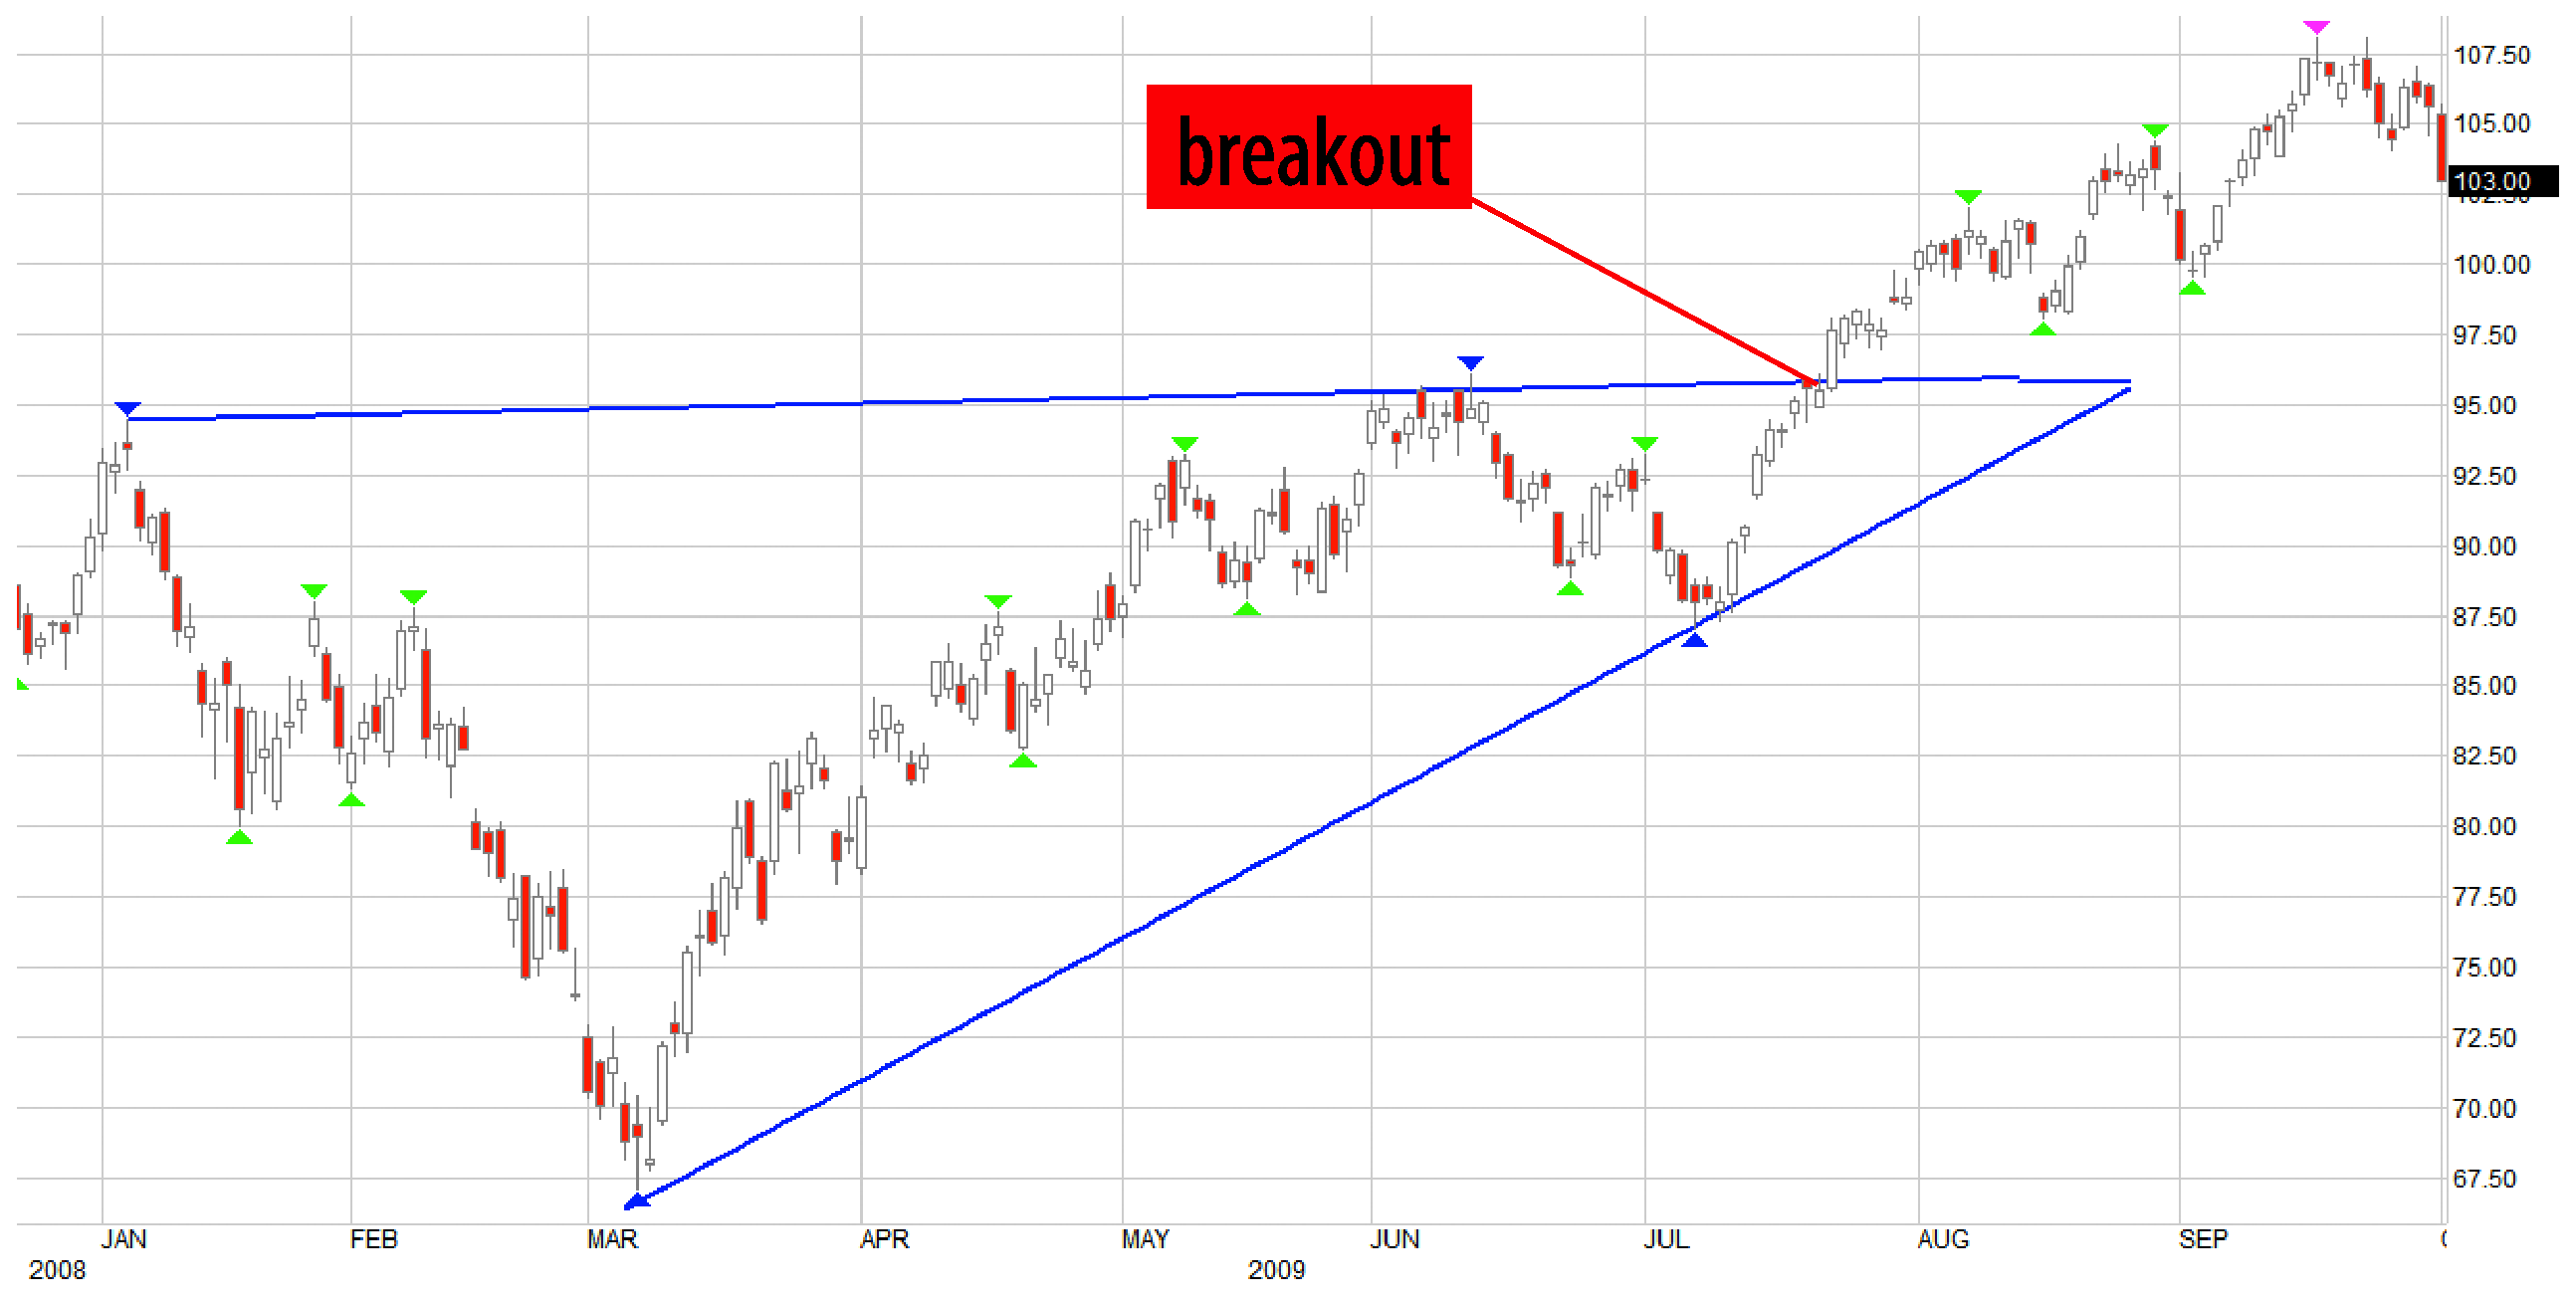
\includegraphics[width=1\textwidth]{figures/Triangle-SPY-1.eps}
\caption{$\mbox{Breakout from a Triangle} SPY \approx 2009$}
\end{figure}
%
\subsection{Accumulation/Distribution}
%
The price of a stock stocks generally show a cyclic behavior, oscillating between a bull and bear market.  During the beginning phase of a bull market, accumulation, the price of a particular stock is low, and considered to be underbought.  Investor interest builds momentum, driving the stock prices higher.  This is the beginning phase of the bear market, distribution, in which the stock price is beginning to reach a point where it is considered to be bought, driving prices down\cite{Bonon}.
\par
One important technique used in technical analysis is being able to predict when a stock is overbought or oversold, before the price signals change direction.  These inflection points in the price signals are known as reversals.  Often, predictive systems are used in technical analysis which attempt to report the current price as a percentage of the accumulation and distribution cycle.  Such measures are known as oscillators \cite{Barbara}.
%
\subsection{Retracement}
%Retracement/Correction/Pullback/Throwback
%
As prices rise (or fall) in a trend, there is a tendency for the price to take a corrective action in the opposite direction (called a retracement), as investors consider that the price may have reached an extreme, triggering an acion to sell (or buy).  After this short-term movement, the stock price then again continues in the direction of the overall trend \cite{Barbara}.  
\par
When purchasing a stock, it is not optimal to pay the highest price the market is willing to ask.  Waiting for the retracement allows investors to purchase a rising stock, at the price it will likely be at a short-term low.
%
\subsubsection{Bullish Retracement}
\label{bullishRetracement}
%
Short-term investors may make use of the retracement in a technique called a bullish retracement.  In this technique the investor wishes to enter a position to take advantage of a bullish trend.  Waiting until a retracement occurs, the stock is purchased at a locally low price.  The stock then again rises with the overall trend, and the investor holds the stock until such time as deemed favorable, when the price has risen above both the retracement price, as well as the original price prior to the retracement.   In this manner, the investor realizes gains since the original stock price, plus the gains from the difference of the original price and the retracement price \cite{Wealth}
\par
A bullish retracement is typically executed as a stop-limit order.  To help ensure the trade is entered during an upward price movement, a stop may be set at a \%ATR above the current price (see Sec.~\ref{ATR}).  Additionally, a limit may be set at some \%ATR below the current price as a way to automatically exit the position if the assumption about the direction of the movement turns out to be incorrect.

%
\subsubsection{Example - Bullish Retracement}
%
Consider ARMH on 20-Oct09 trading around \$7.83 per share.  At this time the ARMH is in a strong upward trend.  The subsequent day, the stock enters into retracement, and continues its downward path until reaching support on 28-Oct-09 at the price of \$7.00 per share.  At this time the stock has an ATR of \$0.23 per share.  If an investor places a stop order one ATR above the current price (\$7.23), the position will be entered when it leaps to \$7.26 on the subsequent day.  If the position is held until it reaches resistance, the sale will be made on 18-Nov-09 at the price of \$8.47 per share.
\begin{center}
\fbox{$(\frac{c_{18Nov}}{c_{28Oct}}-1) \times 100=(\frac{\$7.23}{\$8.47}-1) \times 100=17.15\%\mbox{ ROI}$}
\end{center}
%
\begin{figure}[ht]\centering
\label{fig:retracement}
\includegraphics[width=1\textwidth]{figures/Retracement-ARMH-1.eps}
\caption{$\mbox{Retracement} ARMH \approx 2009$}
\end{figure}



